\documentclass{MScthesisITEM}

% this package is just to generate text for demo-purposes
\usepackage{tipa}
\usepackage{todonotes}
\usepackage{minted}
\usepackage{amsmath}
\usepackage{epstopdf}
\usepackage{pgfplots}
\usepackage{scrwfile}
\usepackage{cprotect}
\usepackage[pdf,tmpdir]{graphviz}


\title{Hybrid Video Topologies} % The title of your assignement; NB use \newlinetitle to start a newline
\author{Tarjei Husøy} % Your firstname and lastname
\professor{Poul Heegaard, ITEM} % Affiliation = ITEM for instance
\supervisor{Svein Willassen, appear.in}

%% Uncomment the following in case you want subfigures; note that there will be a warning for the caption package
\let\subcaption\undefined
\let\subfloat\undefined
\usepackage[width=.85\textwidth]{caption}
\usepackage{subcaption}

\DeclareGraphicsExtensions{.pdf,.eps,.png,.jpg}
\graphicspath{{./figs/}}

\loadglsentries{glossary}
\makeglossaries

\setlength\epigraphwidth{12cm}
\setlength\epigraphrule{0pt}

\lstset{
    showspaces=false,
    showstringspaces=false,
    showtabs=false,
    basicstyle=\footnotesize,
    numberstyle=\footnotesize,
    tabsize=2,
    otherkeywords={with, as},
    language=Python,
    breaklines=true,
    captionpos=t,
}

% CSS driver for LaTeX lstlisting

\lstdefinelanguage{CSS}{
  morekeywords={div,transform},
  morestring=[s]{:}{;},
  sensitive,
  morecomment=[s]{/*}{*/}
}


\pgfplotsset{every axis/.append style={
                    % axis x line=middle,    % put the x axis in the middle
                    % axis y line=middle,    % put the y axis in the middle
                    % axis y line style={<->}, % arrows on the axis
                    % xlabel={$x$},          % default put x on x-axis
                    axis lines*=left,
                    axis x line=center,
                    y axis line style={->}, % arrows on the axis
                    x axis line style={-},
                    ylabel={$y$},          % default put y on y-axis
                    legend style={at={(0.5,-0.10)}, anchor=north,legend columns=-1},
                    major x tick style = {opacity=0},
                    minor x tick num = 1,
                    minor tick length=2ex,
                }}

% \definecolor{blues1}{RGB}{198, 219, 239}
% \definecolor{blues2}{RGB}{158, 202, 225}
% \definecolor{blues3}{RGB}{107, 174, 214}
% \definecolor{blues4}{RGB}{49, 130, 189}
% \definecolor{blues5}{RGB}{8, 81, 156}

% \pgfplotscreateplotcyclelist{colorbrewer-blues}{
%     {blues1},
%     {blues2},
%     {blues3},
%     {blues4},
%     {blues5},
% }

\begin{document}
\listoftodos
\clearpage
\selectlanguage{english}
\pagenumbering{roman}
\pagestyle{plain}

%% Only for the project; comment out the line below for the master's thesis; the front page will be generated automatically by DAIM
%\titleITEM

%% Only for the master's thesis; for the project report the description is taken from It's Learning and added by the department
% \selectlanguage{english} % Change to 'norsk' if you are writing in Norwegian
\begin{titlingpage}

\noindent
\begin{tabular}{@{}p{4cm}l}
\textbf{Title:} 	& \thetitle \\
\textbf{Student:}	& \theauthor \\
\end{tabular}

\vspace{4ex}
\noindent\textbf{Problem description:}
\vspace{2ex}

Current video conferencing services use different topologies and architectures to realize real time communication. One possible architecture, used by the service appear.in, is a full mesh architecture where each participant in a conversation has a full duplex connection with every other participant in the conversation. Another possible architecture, used by many traditional video conferencing services, is to use a Multipoint Control Unit (MCU). This unit will take in video and voice feeds sent from multiple participants which will then be combined into one video/voice feed that can be sent to all participants. This requires decoding and re-encoding of the streams in the MCU. A further possible architecture, is to send all streams through a central Selective Forwarding Unit (SFU), which will forward streams to select participants, based on available bandwidth and other preferences.

The different architectures for video conferencing have different properties. For example, for a conference with only two participants it is usually desirable to use the full mesh architecture, because the direct communication implies lower latency and better quality. However, with growing number of participants requirements on both bandwidth and CPU (due to extensive encoding and decoding) will imply that using full mesh becomes undesirable.  It is therefore likely that the optimal architecture uses a combination of different topologies, depending on the number of participants in a conversation and the resources available to each participant.

The task is to investigate what attributes and requirements a WebRTC conversation needs to perform optimally, and study how different topologies support these requirements.

\vspace{6ex}

\noindent
\begin{tabular}{@{}p{4cm}l}
\textbf{Responsible professor:} 	& \theprofessor \\
\textbf{Supervisor:}			& \thesupervisor \\
\end{tabular}

\end{titlingpage}

\cleardoublepage

%% There must be an abstract in English, even though the main text is in Norwegian
\pagestyle{empty}
\begin{abstract}

Bandwidth efficient, low latencies, cheap -- pick two. This has been the traditional tradeoff for video conferencing providers, where the network topology has limited achiveable performance in many conversation types. Consumers have also suffered under this scheme, as only the biggest companies have been capable of delivering a system that performs in a wide enough range of conversations to grow sustainable. This has limited innovation and made it hard for new providers to enter the market.

This thesis demonstrates how a video conferencing solution can be built using a hybrid network topology, to combine the best properties of peer-to-peer and centralized topologies. For providers utilizing a centralized topology, adopting this work will yield lower costs and better performance for users, while providers utilizing peer-to-peer topologies today can increase the capacity and coverage of their service.

The proposed system dynamically selects the best topology for a given conversation depending on characteristics of each device in the conversation, and will balance routed video to best suit each device. The solution is extendible to include arbitrary characteristics of each device or network link when balancing, and special-purpose nodes like \glspl{sfu} and \glspl{mcu} can further enhance the quality. Each node and link in a conversation is modelled using linear programming (LP), and can be solved by any standard LP-solver. Non-linear properties like queueing delays are approximated by piecewise linear functions.

The peer-to-peer video conference solution appear.in is benchmarked, to see how well peer-to-peer services perform over WebRTC, and to illustrate the potential for a solution that can transcend the boundaries of peer-to-peer. The benchmarking results show severe performance issues for Firefox in constrained conversations, and more moderate potential improvements for Chrome. Tools to assist the benchmarking were developed and is included in the appendices.

\end{abstract}

\cleardoublepage

%% Only for the master's thesis; if the main text is in English and you can write Norwegian, there must be an abstract in Norwegian as well.
\selectlanguage{norsk}
\pagestyle{empty}
\begin{abstract}

Dette prosjektet demonstrerer en videokonferanseløsning basert på en hybrid-topologi, som betydelig øker opplevd kvalitet på tjenesten. For eksisterende tilbydere som baserer seg på sentraliserte nettverk kan denne løsningen senke kostnader og bedre ytelses for brukerne i mange tilfeller. For eksisterende tilbydere som er basert på jevnbyrdsnett så vil denne løsningen øke tjenestens øvre grenser for antall personer som kan være i en samtale.

Systemet vil dynamisk velge den beste topologien for hver enkelt samtale, basert på gitte egenskaper ved enhetene i samtalen.

\todo{Complete this section, less BS and more norsk abstract.}

\end{abstract}

\cleardoublepage

\selectlanguage{english}% Change to 'norsk' if you are writing in Norwegian

\renewcommand{\abstractname}{Acknowledgements}
\begin{abstract}

I want to thank my supervising professor at \gls{item}, Poul Einar Heegard, for <snip>, and Svein Willassen, my supervisor at appear.in who proposed the topic.\todo{Finish writing acknowledgements}

\end{abstract}

\cleardoublepage

\tableofcontents*
\cleardoublepage

%% include if relevant
\listoffigures
\cleardoublepage

%% include if relevant
\listoftables
\cleardoublepage

%% include if relevant
% \listofalgorithms
% \addcontentsline{toc}{chapter}{List of Algorithms}
% \cleardoublepage

%% include if relevant
\printglossary[title=List of Symbols, style=long]
\cleardoublepage
\glsaddall[]

%% include if relevant
\printglossary[title=List of Acronyms,type=\acronymtype] % prints just the list of acronyms
\cleardoublepage

\pagenumbering{arabic}
\pagestyle{ruled}

%% What's the problem, considerations that need to be taken, etc
\chapter{Introduction}\label{chp:introduction}

The web is becoming the primary platform for all communication, as people gradually move away from the solutions provided by their telco operator, such as telephony and text messaging. Moving audio conversations to the Internet has been relatively easy, but as we're now commoditizing video conversations, moving away from custom rooms and dedicated hardware over the regular laptops and phones, the most straightforward solutions lead to performance requirements greater than most user equipment and their connections can handle.

There are lots of competing products on the market today, with different characteristics and performance levels. What they all have in common however, is that they've all chosen a fixed network topology, which dictates most of their expected performance. The goal of this thesis is to investigate the feasibility of designing a system which does not have a fixed topology, but choses one adaptively based upon properties of the user equipment and connection quality in a given conversation.

\todo[inline]{Write about what WebRTC is how that changes the playing field for real-time communication}

The goal of this project is to maximize user utility in video conference solutions. To maximize utility, we need to have a well-defined sense of what that implies.


\section{Context and utility}

When defining user utility, context is everything. You have different expectations to audiovisual quality on a desktop computer with fiber connectivity compared to your phone on 3G. But how can this difference be quantized? Certainly it's not a question of screen resolution, as most smart phones today have the same 1080p resolution as most computer screens. Resolutions beyond 1080p, like we can find on some "retina" screens, are not that interesting for video conferencing, as the webcam producing the source video is unlikely to be able to keep pace.

However, physical screen size matters. Viewing distance matters. Latency matters very much. Bandwidth matters. Packet loss matters. Most of these should be fairly easy to estimate, but then we have a new problem: which of these attributes do we prioritize? Finding the optimal balance is the key to optimizing user utility. There are of course also non-technical factors that affects the expected experience quite much that cannot be determined by the device itself. For example, even though the device is the same, you'll have different expectations sitting on the bus to work compared to sitting in a sofa in your living room, even though the device and maybe even the connection is the same. Content matters. Environment matters. Mood matters. Time of day probably matters. We will however not take all of these factors into account, but limit our scope to the device and the connection, and since the intended application is to WebRTC, what we can relatively easy determine through the browser.

There will also be diminishing returns on most of these metrics. If you have practically unlimited bandwidth available, there's little to gain from sending video with bitrates in excess of 3 Mbps, you'll just be wasting bandwidth, CPU and battery. If we define a quality threshold for a device as the "optimal" experience that can be attained as 1.0, there's no reason to try to push this as high as possible. We can though assume that all metrics that are lower than what's necessary for this optimal experience will subtract from this quality metric somehow. For example, if we say that the threshold for optimal latency for a device is \(20ms\), we can imagine a \gls{utility function} that behaves like \(1 - x^t\), where t is a constant determining how fast this metric deteriorates. The general function is illustrated in \autoref{fig:utility-latency}.

\begin{tikzpicture}
    \begin{axis}[
        xlabel={$t (ms)$},
        ylabel={$f(x) = 1 - x^t)$},
        xmin=0,
        ymin=0,
        ymax=1,
        xmax=250]

    \addplot+[domain=0:250]{0.6 + 0.4*rad(atan(20*0.1 - 0.02*x))};
    \label{fig:utility-latency}
    \end{axis}
\end{tikzpicture}

For now we'll assume that we have a function similar to the one illustrated in \autoref{fig:utility-latency}, returning a value approximately in the range \todo{Find the proper lower limit}\(1 -- 0\), for each of the metrics that comprise the user utility. Multiplying these together we'll get a user utility that lies in the same range.

Assuming this user utility function, we have to figure out what to optimize in a conversation. If a single party in a conversation experiences high latencies and much packet loss, it's likely to negatively affect the experience of all the other parties as well, due to that person requesting people to repeat what they said and being hard to hear for other participants. We'll thus focus on maximizing the minimum utility experienced in a conversation, and then gradually improve the utility for all users ordered by their current utility in ascending order.


\section{Previous and Related Work}

\epigraph{If I have seen further, it is by standing on the shoulders of giants}{Isaac Newton}

Networking and algorithms related to networking is not a new topic, by any stretch of the imagination, and like in all most branches of computer science, it's mostly old problems in a new context.

During this thesis we will borrow heavily from previous work on networking and graph algorithms in general, and flow algorithms in particular. Many algorithmic problems can be solved as a linear program, which as a problem was first solved by Fourier in 1827\cite{sierksma2001linear}. Another solution, the simplex method, was first introduced by G.B. Dantzig in 1947\cite{sierksma2001linear}, and was first introduced to me in \cite{ahuja1988network} by Ahuja, Magnanti and Orlin, and serves as the basis for much of our suggested solution. The simplex method has been widely adopted for its ease of implementation on computers, and years of exponential growth of computer performance has made increasingly large problem sets solvable in realistic time.

Now that we've established the problem domain and have some grasp of the main challenges, let's see where we are today.


\section{Disclaimer}

This thesis does not try to measure or optimize for audio transmission, as that's a much simpler problem that can practically always be completed by sending the same stream to all nodes in the conversation. There's always only one stream to encode, it doesn't noticably affect available bandwidth, and it's already widely deployed. However, results we achieve for video can also be applied to audio streams if the environment is very heavily constrained or further optimization is required, it's just not the focus of this thesis.


%% Look at some technical aspects, introduce current providers
\chapter{Background}
\label{chp:background}

In this chapter we'll first discuss some technical aspect of video conferencing that affect how we reason about solving the challenges, before performing we try to benchmark existing solutions to see how they perform in our example conversations.


\section{A technical look at video conferencing}

\subsection{Codecs}

\todo[inline]{Write about the future of H.264/VP9, SVC, hardware acceleration, etc}

\subsection{CPU limitations}

The naïve approach to encoding the videostreams is to encode the raw stream from the web camera into several client-optimized streams for transmission. Using VP8, this is the only way to do it. However, H.264 can be encoded in a \gls{svc} manner, which makes it possible to extract different bandwidth-streams from a single stream. With VP8 this is sadly not possible, and the only alternative is to utilize a \gls{sfu}, a technique where several streams are sent to the same endpoint, which can then select which of the streams to forward to the different endpoints. This is not as efficient as sending only a single stream however, and the encoding step is also costlier on the CPU.

\subsection{Continuous Presence}

\todo[inline]{Only do Continous Presence if the client has enough available bandwidth, ie $BW_{down}>(n-1)*BW_{min}$, otherwise fall back to \gls{vas} through an \gls{mcu}}

\todo[inline]{Write about Continuous Presence (multiple parties on-screen at the same time), and how that limits the different topologies}

\todo[inline]{Could the problem be avoided by not using continuous presence for challenged parties? Like only receiving a single stream from the talking party, and get some sort of indication from the network who is talking? Uploads would still have to be solved though..}


\section{The current providers}

Now that we have established our example conversations, we can turn to see how they'll behave in the solutions available today. The most popular video conferencing solutions available today are:

\begin{center}
	\label{tab:existing-solutions}
	\begin{tabular}{| l | l |}
		\hline
		\textbf{Service} & \textbf{Description} \\ \hline
		appear.in & Peer-to-peer WebRTC service \\ \hline
		Google Hangouts & Browser-based service utilizing a Google MCU \\ \hline
		Microsoft Skype & Downloadable app, closed source protocol \\ \hline
		Cisco TelePresence & Custom hardware, self-hosted or cloud service \\ \hline
	\end{tabular}
\end{center}

Notably absent here is FaceTime, Apple's videochat service bundled with their devices. FaceTime's absence in this thesis is due to the lack of support for more than two people in a conversation, which makes the optimal topology question embarassingly easy to answer, and the lack of support on non-Apple devices, which makes the service uninteresting.

We also note that Mozilla just entered the market in collaboration with Telefonica with their Hello service, bundled with recent versions of Firefox\footnote{https://www.mozilla.org/en-US/firefox/hello/}. Hello however essentially provides the same service as appear.in, just bundled with the browser. Thus anything we say about appear.in applies to Firefox Hello as well, and we'll therefore not consider them separately. This author will however congratulate Mozilla and Telefonica on their endeavor to make communication more open and available to anyone.

Let's take a more detailed look at these services.

\subsection{appear.in}

\todo{Write appear.in background}


\subsection{Google Hangouts}

Google Hangouts is alongside appear.in the only other service based in the browser. Hangouts is a merge of several earlier Google communication solutions like Google Talk, Google+ Messenger and the Hangouts feature from Google+. The service uses a Google-provided \gls{mcu}, and VP8/9 over WebRTC as video transport\todo{Find a source to verify this}. A conversation is limited to 10 people.

To use Google Hangouts it requires you to setup a public Google+ profile, which makes the barrier of entry significantly higher than for some of the other services tested in this thesis. It also requires installing the Hangouts extension for video conferencing to work.

In our test scenarios, Google Hangouts performs like this:

\todo[inline]{Get test data from hangouts}


\subsection{Skype}

Skype is probably the most well-known of the solutions we're looking at, being the first to offer free video conferencing for personal use. Skype was also among the first to provide a VoIP solution interoperating with \gls{pstn}, easing the barrier of entry for new users. The original Skype topology was peer-to-peer, routing streams through PCs with Skype installed that had the app running, using a proprietary closed-source protocol. After the Microsoft aquisition Skype ditched the peer-to-peer design to a Microsoft MCU-backed solution, justified as a means to improve performance and security for users. A Skype conversation has a soft limit on five people for the best user experience, hard limited to 10 users.

Skype requires a standalone application to run, which is available on pretty much every platform out there, including Windows, Mac, Linux, Android, iOS, Windows Phone, BlackBerry, most tablets, TVs, gaming consoles and more. The benefit is close access to hardware and GPUs for more efficient video encoding, the downside is the lack of open protocols and standardization.

Skype performance summarized:

\todo[inline]{Add skype test data}


\todo{Which providers do we have today and what sort of topologies do they use? What are their pros and cons?}



\section{Where we want to be}

\todo{What is the intended outcome of this work?}


\section{Related Work}

\todo{What other work in this area have we learned from and built upon?}

A study at Chalmers in 2014\cite{tree-topology-webrtc} investigated the feasibility of utilizing normal nodes in a video conference as supernodes, routing traffic from less powerful nodes through these nodes to reduce network load. The authors conclude that such a solution is feasible given proper supernode selection, which gives even greater possibilities for a solution utilizing dynamic topologies like presented in this thesis. Pushing as much traffic as possible over client-provided supernodes lowers the cost for the provider, and enables better quality for the users since peers can be closer to each other than to the closest data center.


%% introduce the test cases
\chapter{Test Cases}\label{chp:test-cases}

To narrow down the problem scope a little, I'll define some test cases we can work on, and assume that if a solution can efficiently serve these cases, it can serve most others as well. A summary of the test cases are given in \autoref{tab:test-cases}. Note that these are intended to be hard cases, with at least one node being more significantly more constrained than the others. Thus, failure to pass these tests do not necessarily imply that the solution is useless, only that there are cases where it'll fail, or perform sub-optimally. \autoref{fig:test-cases} illustrates the test cases graphically with the all the inter-node latencies.

\begin{center}
    \captionof{table}{Test Cases}
    \label{tab:test-cases}
    \begin{tabular}{| l | l | p{7cm} |}
    \hline
    \textbf{Case name} & \textbf{$n$} & \textbf{Description} \\ \hline
    Traveller & 3 & Two people with decent connections between them, one remote with high latency and severely restricted bandwidth to the others. \\ \hline
    Standup & 4 & Two people on desktop machines with wired connections, one laptop and one tablet on WiFi. \\ \hline
    Friends & 7 & Group split in two locations, each subgroup having short latencies internally, but larger latencies to the other group. Heterogenous bandwidths across the board. \\ \hline
    \end{tabular}
\end{center}

How realistic are these cases? According to the appear.in data set in \autoref{chp:appear.in-usage}, \todo{Complete rationalisation of test cases}.

Are there any trivial cases that can be ignored? As long as there's only two people in a conversation, and they have fairly low latency between each other and sufficient bandwidth, peer-to-peer is the optimal choice in all cases. Initially, it might seem like this would indeed be the case in all conversations with two participants, and not just the good-bandwidth, small-latency onces. However, this is not the case. To illustrate why, consider a conversation between two people, one in Europe and one in Asia. The \gls{rtt} between them is ~350ms. They both have fairly acceptable bandwidth, with 3Mbps each, which should be plenty to sustain an acceptable video link between them. This might not be the case, as the bandwidth between them is far more limited due to the long distance and many hops through publicly routed networks. But if each of the peers has a data center of a distributed VPS provider nearby, to which they can utilize their full bandwidth, this limitation might be overcome. These distributed VPS providers tend to have established high-quality routes between their own data centers, backed by \glspl{sla} and much higher bandwidths than available to private entities.

The available bandwidth between the two data centers is thus far greater than what can be achieved directly between the two peers. Because of this, their video link can be improved by routing their traffic through the data centers, thus enabling each peer to utilize the full bandwidth of their connection.\footnote{This is backed by a simple experiment, using DigitalOcean as our VPS provider. From a 100Mbit university connection in Norway, sustained data rates to their Singapore data center varied greatly, measuring 90kBps, 3,7MBps, 1,9MBps and 2,58MBps for each test. However, from their Amsterdam data center, a consistent throughput of 24,6MBps was measured}. The latency though is close to unchanged from routing through the data centers, only sustained bandwidth between the peers is improved (and probably less packet loss).

These conversations are not extensive, but should cover enough corner cases to be able to highlight the pros and cons of the different topologies. The examples cover the low-latency, few peers conversations; the bandwidth-challenged cases; the high-latency conversations; and the very heterogeneous device conversations, where one or more party is severely challenged in terms of either bandwidth or latency.

We assume that the back-end networks are not saturated, and that each user is bandwidth-constrained only by their connection. By extension, the maximum bandwidth attainable between any pair of nodes in our network is the lesser of the upload bandwidth of the sending party and the download bandwidth of the receiving party. However, latency has to be defined for any pair of the nodes in the network, as this is mostly determined by their geographical location in relation to each other. To best illustrate the physical topology, we can draw each scenario as a complete graph:

\begin{figure}
    \begin{subfigure}{\textwidth}
        \centering
        \includegraphics{test-case-traveller}
        \subcaption{Test case ``traveller''.}\label{fig:test-case-traveller}
    \end{subfigure}

    \begin{subfigure}{\textwidth}
        \centering
        \includegraphics{test-case-standup}
        \caption{Test case ``standup''}\label{fig:test-case-standup}
    \end{subfigure}

    \begin{subfigure}{\textwidth}
        \centering
        \includegraphics[width=\textwidth]{test-case-friends}
        \caption{Test case ``friends''}\label{fig:test-case-friends}
    \end{subfigure}
    \caption{The different test cases}
    \label{fig:test-cases}
\end{figure}


%% Benchmark the existing providers to figure out where the bar lies
\chapter{Experiments}\label{chp:experiments}

In this chapter we'll benchmark a WebRTC-based video conferencing solution for our test cases, to get a sense of how a peer-to-peer architecture performs.


\section{Test Setup}

To benchmark appear.in, our WebRTC-based video conferencing solution of choice, we have utilized a small cluster of desktop computers with web cameras, running the most recent versions of Mozilla Firefox\footnote{Version 36.0.4, latest version as of 2015.06.05 when the tests were run} and Google Chrome\footnote{Version 41.0.2272.101, latest version as of 2015.06.11 when the tests were run}. These two browsers were chosen since they collectively represent 85\% of the browser market (according to both appear.in data as seen in \autoref{chp:appear.in-usage} and the W3C \cite{browser-stats}), and are powered by two different underlying engines. The goal of the benchmark is to get a sense of how the browsers -- and by extension, appear.in -- performs with regard to latency and bandwidth usage in our different test scenarios, and from that data observe how resources are shared among the nodes in a conversation.

Since the test covers two different browsers which do not share a common API (more on this later), measurements were done in two different ways. For Firefox, which do not expose timing data of WebRTC-streams, a browser-external way of measuring end-to-end latencies was necessary. For this we synchronized all the clocks in the cluster to the same \gls{NTP} server, and set another independent node -- also synced to the same time server -- to run a timer. Each of the nodes in the test filmed this timer, and with the same timer running locally in a terminal, the end-to-end latency could be extracted by taking regular screenshots, and finding the difference between the local timer and the timer as sent by the other nodes. See \autoref{fig:example-screenshot} for an example of how the screenshots looked.

\begin{figure}
    \centering
    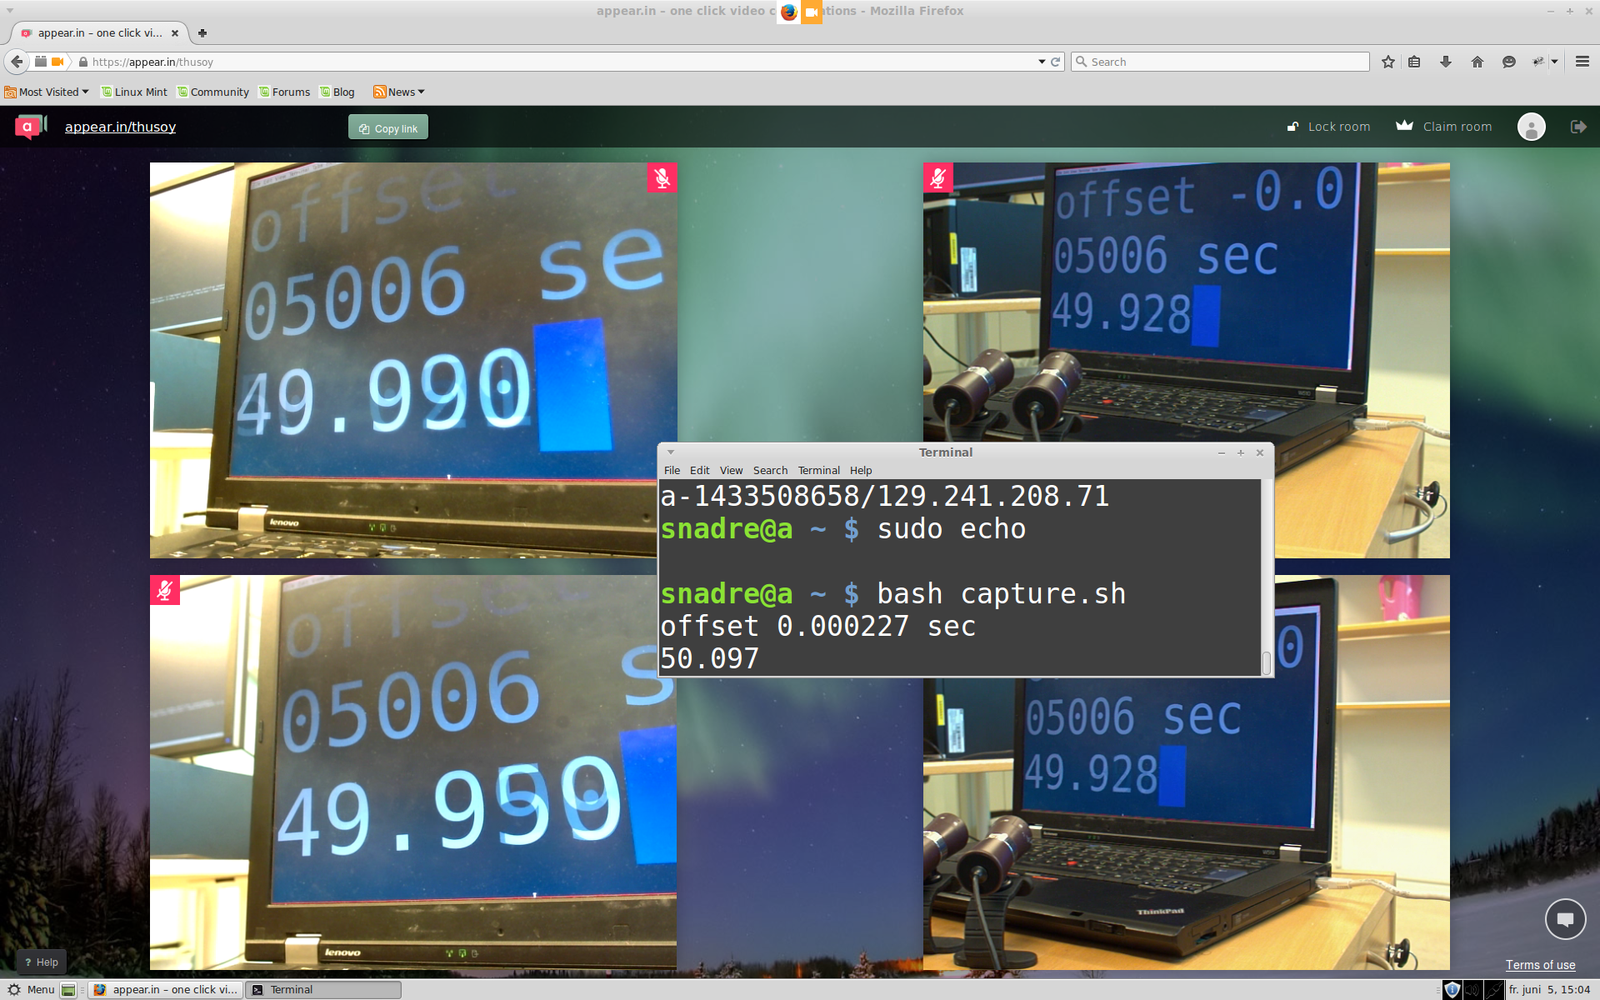
\includegraphics[width=.7\textwidth]{example-screenshot}
    \caption{An example screenshot from a test run on node A. The nodes are, from top left and clockwise, A, C, B and D. We can see from the difference between the local timestamp and A's own video stream that there's about 75ms of processing time in the browser before the image is sent (if we round A up to the almost visible 50.021 timestamp), and that the latencies from the other nodes are 31ms, 93ms and 93ms for B, C, and D, respectively.}
    \label{fig:example-screenshot}
\end{figure}

Bandwidth usage was measured by running \texttt{tcpdump} throughout the test run, and later extracting sent and received data with \texttt{tshark}.

For the Chrome tests, this was a bit simpler and less manual, as Chrome do provider timing data through the \texttt{getStats} API. Firefox also supports \texttt{getStats}, but does not return as much data as Chrome does, even though the data is assumed to be available internally in the browser.


\subsection{Sampling}

At the start of the test, the nodes join the conversation in alphabetical order (the node names are letters A-G), as soon as the previous node has established connection to all the other parties already in the conversation. Preferably the join order would be random and the results averaged over several test runs, but due to time constraints this was not possible.

When all nodes have established bi-directional connections, the conversation was left running for a minute, before sampling started. This was done to allow some time to reach a stable state.

For Firefox, where the interpretation of the results is a very tedious and laboursome process, samples were taken every $\approx$12s\footnote{A bit variable, as it's 10s + the delay for taking and storing the screenshot}. The last six samples for each node was interpreted and stored, yielding a total sample time of $\approx$80s. On Chrome, were there's no interpretation step, samples were submitted every second, and the sample time was two minutes, yielding 120 samples for each node.

For all test cases the test was first run without any traffic shaping applied, so that the actual test results could be seen in comparison to results without any network limitations.


\subsection{getStats}

The relevant values offered by the \texttt{getStats}-API on Chrome\footnote{Documentation is very poor for the \texttt{getStats}-API, as the specification is not completed yet, so the most reliable reference is the source: \url{https://chromium.googlesource.com/external/webrtc/+/master/talk/app/webrtc/statstypes.cc}} and Firefox is presented in \autoref{tab:incoming-video} and \autoref{tab:outgoing-video}. The values reported here were dumped from what's returned by the browser.

\begin{center}
    \captionof{table}{Incoming video data}
    \label{tab:incoming-video}
    \begin{tabular}{| l | l |}
        \hline
        \textbf{Chrome} & \textbf{Firefox} \\ \hline
        \multicolumn{2}{| c |}{bytesReceived:\texttt{str/int}} \\
        \multicolumn{2}{| c |}{packetsLost:\texttt{str/int}} \\
        \multicolumn{2}{| c |}{packetsReceived:\texttt{str/int}} \\ \hline
        googCurrentDelayMs:\texttt{str} & jitter:\texttt{float} \\
        googDecodeMs:\texttt{str} & mozRtt:\texttt{int} \\
        googJitterBufferMs:\texttt{str} & \\
        googMaxDecodeMs:\texttt{str} & \\
        googMinPlayoutDelayMs:\texttt{str} & \\
        googRenderDelayMs:\texttt{str} & \\
        googTargetDelayMs:\texttt{str} & \\ \hline
    \end{tabular}
\end{center}

\begin{center}
    \captionof{table}{Outgoing video data}
    \label{tab:outgoing-video}
    \begin{tabular}{| l | l |}
        \hline
        \textbf{Chrome} & \textbf{Firefox} \\ \hline
        \multicolumn{2}{| c |}{bytesSent:\texttt{str/int}} \\
        \multicolumn{2}{| c |}{packetsSent:\texttt{str/int}} \\ \hline
        googAvgEncodeMs:\texttt{str} & bitrateMean:\texttt{float} \\
        googCaptureJitterMs:\texttt{str} & bitrateStdDev:\texttt{float} \\
        googCaptureQueueDelayMsPerS:\texttt{str} & droppedFrames:\texttt{int} \\
        googCodecName:\texttt{str} & framerateMean:\texttt{float} \\
        googBandwidthLimitedResolution:\texttt{str} & framerateStdDev:\texttt{float} \\
        googCpuLimitedResolution:\texttt{str} & \\
        googViewLimitedResolution:\texttt{str} & \\
        googRtt:\texttt{str} & \\
        packetsLost:\texttt{str} & \\ \hline
    \end{tabular}
\end{center}

It's a bit sad to see that all of the values are casted to strings in Chrome. This is not the case on Firefox, where appropriate types are used. As we also see, all of the timing-related values we're interested are vendor-prefixed on Chrome, which hints to their unspecified nature. Note that both browsers report more data than what is shown here, this is only the data I consider to be relevant for our bandwidth and latency measurements (and link quality, thus the ones related to packet loss). Chrome is also very helpful in providing why resolution is limited (received resolution is present in the full data set), which could be incorporated into more advanced models.


\subsection{Constraining Nodes}

To configure the cluster according to the different test cases, we utilized the Linux traffic control utility \texttt{tc}, which is capable of rate-limiting incoming and outgoing traffic, as well as delaying traffic destined for certain hosts. A small script was developed to act as a glue layer between a representation of a network and \texttt{tc}, making configuration repeatable and easily parametrized. The script is included in \autoref{chp:apply-case}. The test cases from \autoref{chp:test-cases} was serialized into \gls{yaml}, and the same case definitions could then be used by both the script configuring the nodes, and for the sample solution provided in \autoref{chp:suggested-solution}.

Applying a given test case is thus completely independent of the actual network utilized in the test cluster, keeping all intelligence on the nodes themselves. This removed the need for expensive routers or having to customize the application code, thus making the method application agnostic and applicable to any peer-to-peer solution, not just appear.in.


\subsection{Automated Testing?}\label{subsec:automated-testing}

Ideally, testing would be automated and not require a running graphical environment, to allow tests to be run often and in response to events such as commits. This could be possible using by running a browser in a fake framebuffer like \texttt{Xvfb}\footnote{\url{http://www.x.org/releases/X11R7.6/doc/man/man1/Xvfb.1.xhtml}} and faking out a media stream\footnote{Chrome: \texttt{-{}-use-fake-device-for-media-stream}, Firefox: \texttt{getUserMedia(\{fake: true, <...>\})}. More info about this approach can be found at \url{http://images.tmcnet.com/expo/webrtc-conference/presentations/san-jose-14/D3-2_Testing_v2_2.pdf}}. Both browsers should be able to be tested in such a setting, but data would be limited to what can be extracted through the \texttt{getStats}-API as described above. Still, it's better than nothing. It is thus possible to automate this, but was considered out of scope for this thesis.

Chrome runs regular interoperability tests with Firefox\footnote{Google blogged about this: \url{http://googletesting.blogspot.se/2014/09/chrome-firefox-webrtc-interop-test-pt-2.html}}, but these tests only test that calls can be established, and do not test any network configurations or measure statistics. Integrating the results from this thesis into this test suite is encouraged for more insight into the performance and behavior of WebRTC implementations. The W3C also maintain a test suite for implementations\footnote{\url{http://www.webrtc.org/testing/w3c-conformance-tests}}, but those only test compatibility with the APIs, and not network behavior.


\subsection{Caveats}

The Firefox method is accurate in the sense that latencies observed are the actual end-to-end latencies that users would observe, but the precision of the timing values observed is not on the millisecond level we'd prefer. This is due to a number of factors, most notably the refresh rate of the screen running the timer and the framerate of the video, limiting the precision to $1s/60\approx17ms$ and $1s/30\approx33ms$ respectively. However, we can surpass this precision by averaging several samples taken during the test run, which is why we take several screenshots for each test case, once every 10s for at least a minute. The standard deviation of the measurements is reported in the graphs included later in this chapter, which should give some indication towards how accurate the average is.

Taking several samples to improve accuracy leads us to another weakness, which is the manual interpretation of the screenshots. Due to the frequency-related issues discussed above, many of the images include timestamps that are blurred, as the camera captured two underlying screen updates in the same frame, as shown in \autoref{fig:blurred-capture}.

\begin{figure}
    \centering
    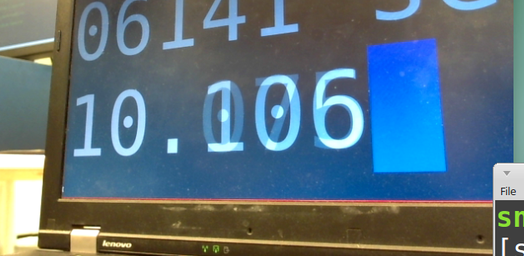
\includegraphics[width=.7\textwidth]{blurred-capture}
    \caption{A screenshot where a node has sent two overlaying timestamps. In this case interpreted as 10.106, which is reasonable as it's close to the expected 33ms increase from the previous 10.075.}
    \label{fig:blurred-capture}
\end{figure}

In general for these cases, the recorded timestamp was consistently interpreted to be the latest of what could be distinguished in the screenshot.

Even assuming that the timestamps are comprehensible and fairly accurate, there's still a possibility of human error when lots of numbers has to be recorded in this way. To minimize the risk of any mistyped numbers making it into the dataset, any number outside 1.5 standard deviations of the mean (a range which should include 87\% of the numbers observed) was verified once more. There's still a chance of smaller errors making it into the dataset, but we assume that these are small enough and distributed evenly among the nodes to not significantly influence any conclusions drawn.

As not enough cameras of any single model was available for the experiments, two different models\todo{Insert picture of the cameras here, or footnote} had to be used. These had slightly different performance characteristics; the cameras were put side by side with a timer and showed a mean difference of 39.6ms, but with a relatively large standard deviation of 19.5ms. As the same restrictions on screen refresh rates as discussed above, pretty much all the samples were at a 30ms or 60ms interval of each other.\footnote{Out of 20 samples, 1 was 0ms, 13 were 30ms, 5 were 60ms, and 1 was 90ms. Which really means in the range of that frame, that is in the range of 0--29ms difference, 30--60ms difference, and so on.} As the difference was assumed to be normally distributed, the mean was simply added to all measurements from the slower camera model to compensate.

For measuring bandwidth utilization between nodes, our method of using \texttt{tcpdump} is not entirely satisfactory, as there's no way to report actual \emph{consumed} bandwidth by the application. This is because the traffic control features of the Linux kernel lies above \texttt{libpcap}, the library that performs packet capture for \texttt{tcpdump} in the network stack. Effectively this means that any incoming bandwidth reported by \texttt{libpcap} will be before the rate limiting performed by \texttt{tc}. Thus, \texttt{tcpdump} cannot report the actual bandwidth consumed by application, only what was received by the network interface. Nonetheless, the bandwidth \emph{sent} by each node is what was actually sent by the application, but there's no guarantee that the receiver was capable of consuming it all. This is good enough for us though, as we can aggregate the data sent by all nodes to determine how saturated a given node's network link is.

While the method itself is application-agnostic, configuring nodes the way we do is not suitable for testing other architectures, such as the ones used by Hangouts and Skype. This is unfortunate, as a performance comparison between the different architectures would have been very interesting, but without running a local instance of the architecture under test, there's no way to achieve the inter-node latencies we desire. This follows from observing that if node A sends her video stream to a Google server, there's no way for her to signal to Google that when the stream is broadcast to nodes B and C, B's stream should be delayed by $x$ ms, and the stream to C should be delayed $y$ ms. It's also not possible for B and C to apply this latency on the receiving side, as they'd have to split the incoming stream for Google into separate streams for each of the transmitting nodes, which would require both getting access to the DTLS keys used by the web browser to encrypt the traffic, and being capable of splitting the stream and rejoining it again without interfering with the browser.

For the most accurate comparison of bitrate, it would have been preferable to use the same method for sampling this on both browsers. However, as Firefox was incapable of delivering timing data, the \texttt{getStats} API was discarded entirely, even though it could have been used to sample bitrates as observed by the application. This is unfortunate, but the tools left behind by these experiments allow others who want to repeat the tests to not do this mistake.


\section{Results}

\subsection{How To Read the Graphs}

As there will be a lot of graphs in this chapter, a good understanding of how to read them is essential. \autoref{fig:graph-tutorial} gives you a quick primer.

\begin{figure}
    \centering
    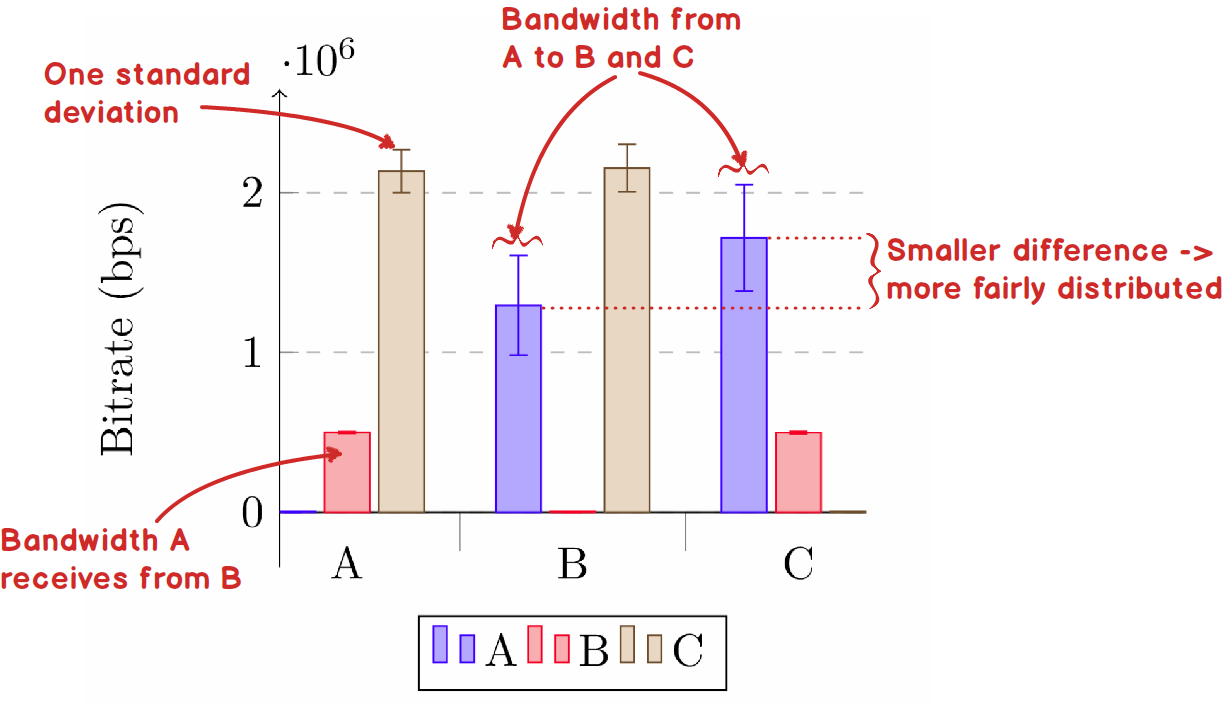
\includegraphics[width=\textwidth]{graph-tutorial}
    \caption{How to read bandwidth graphs. Latency graphs are the same, just different units.}
    \label{fig:graph-tutorial}
\end{figure}

For each node on the x-axis, if it's a latency chart the node's happier the more of the latencies are low. If it's a bitrate chart, the node's happier the more of the bars are high.

Before we embark on the test cases, we put our two sampling methods up against each other, to see whether the results are comparable. For each of the conversation sizes, 3, 4, and 7, the results were equal across the board for both browsers. Both had a consistent stable bandwidth at slightly less than 2.1Mbps, and latencies below 200ms (Chrome slightly less). The results are included in \autoref{no-shaping-comp}.

\todo[inline]{[minor] If time, define custom color set for graphing, based possibly either on solarized or http://clrs.cc/}

\subsubsection{Test Case ``traveller''}

A quick recap of the bandwidth limits put on the nodes in the ``traveller'' test case: A (10/5), B (2/1), C (10/8).

\autoref{fig:traveller-bitrate} shows the bitrates flowing between the nodes in the ``traveller'' test case. Remember what was mentioned earlier; the values reported here are only what was received at the node's interface, not what the application was consuming. This is important, as it seems from the bandwidths alone that everyone is doing fairly well in the Firefox case; but look closer. Node B only has a 2Mbps downlink, but is sent more than 3Mbps of data. Thus its link is completely saturated, which is again reflected in the latencies in \autoref{fig:traveller-latency}. We can also see that node B is saturating its own uplink as well, which also has a grave impact on the latencies.

Chrome balances this out much better, where A and C communicate unhindered by the constraints of node B (like the Firefox case), but also respect B's constraints and only send what it's capable of receiving. Thus, B's downlink has $\approx$50\% utilization, and likewise $\approx$66\% for the uplink.

\begin{figure}
    \centering
    \begin{subfigure}[t]{.48\textwidth}
        \centering
        \begin{tikzpicture}
        \begin{axis}[
            ybar,
            ylabel=Bitrate (bps),
            xtick=data,
            width=\textwidth,
            symbolic x coords={A,B,C},
            enlargelimits=0.15,
            major grid style=dashed,
            ymajorgrids,
            ]
            \input{data/appear.in-traveller/bitrate.tex}
        \end{axis}
        \end{tikzpicture}
        \subcaption{Firefox}
    \end{subfigure}
    \hfill
    \begin{subfigure}[t]{.48\textwidth}
        \centering
        \begin{tikzpicture}
        \begin{axis}[
            ybar,
            compat=newest,
            ylabel=Bitrate (bps),
            xtick=data,
            width=\textwidth,
            symbolic x coords={A,B,C},
            enlargelimits=0.15,
            major grid style=dashed,
            ymajorgrids,
            ]
            \input{data/appear.in-final-traveller/bitrate-getstats.tex}
        \end{axis}
        \end{tikzpicture}
        \subcaption{Chrome}
    \end{subfigure}
    \caption{Observed bitrates in the ``traveller'' test case}
    \label{fig:traveller-bitrate}
\end{figure}

\begin{figure}
    \centering
    \begin{subfigure}[t]{.48\textwidth}
        \centering
        \begin{tikzpicture}
        \begin{axis}[
            ybar,
            ylabel=Latency (ms),
            xtick=data,
            ymax=1000,
            width=\textwidth,
            symbolic x coords={A,B,C},
            enlargelimits=0.15,
            major grid style=dashed,
            ymajorgrids,
            ]
            \input{data/appear.in-traveller/latency.tex}
        \end{axis}
        \end{tikzpicture}
        \subcaption{Firefox}
    \end{subfigure}
    \hfill
    \begin{subfigure}[t]{.48\textwidth}
        \centering
        \begin{tikzpicture}
        \begin{axis}[
            ybar,
            compat=newest,
            ylabel=Latency (ms),
            xtick=data,
            ymax=1000,
            width=\textwidth,
            major grid style=dashed,
            ymajorgrids,
            symbolic x coords={A,B,C},
            enlargelimits=0.15,
            ]
            \input{data/appear.in-final-traveller/latency-getstats.tex}
        \end{axis}
        \end{tikzpicture}
        \subcaption{Chrome}
    \end{subfigure}
    \caption{Observed latencies in the ``traveller'' test case. Actual values for the out-of-bounds values in Firefox, from left to right: 26s, 48s, 48s, 23s.}
    \label{fig:traveller-latency}
\end{figure}


\subsection{Test Case ``Standup''}

Quick refresher on ``standup'' bandwidth limits: A (30/20), B (30/15), C (8/6) and D (6/3).

The key challenge in this case is node D, with only 6 Mbps available on the downlink, slightly upped by node C with 8 Mbps. Observed bitrates from the test are given in \autoref{fig:standup-bitrate}. Firefox displays much of the same things we saw for the ``traveller'' test case; Node C doesn't have any troubles in this test, but node D is completely saturated. Node D receives 2.1 Mbps from each of the other three nodes, which again destroys the latencies in the conversation. Even though node D sends to its fullest capacity, hardly anything of this is correctly received by the other nodes. This probably implies that among the data Firefox is actually putting onto the wire, not enough of it reaches the destinations unfragmented, and thus the receiver is incapable of reconstructing a complete frame to show to the user. Node C doesn't entirely saturate it's uplink however, so there's obviously \emph{some way} streams are limited in Firefox, but it's clearly not adequate.

Chrome handles the two challenged nodes elegantly, with 61/76\% downlink/uplink utilization on node C, and 85/80\% utilization on node D. The complete link utilization results are given in \autoref{tab:utilization-standup}.

\begin{center}
    \captionof{table}{Link utilization in the ``friends'' test case}
    \label{tab:utilization-standup}
    \begin{tabular}{| l | l | l |}
    \multicolumn{3}{c}{\textbf{Firefox}} \\ \hline
    \textbf{Node} & \textbf{Downlink} & \textbf{Uplink} \\ \hline
    \input{tmp/standup-utilization-firefox}
    \hline
    \end{tabular}
    \begin{tabular}{| l | l | l |}
    \multicolumn{3}{c}{\textbf{Chrome}} \\ \hline
    \textbf{Node} & \textbf{Downlink} & \textbf{Uplink} \\ \hline
    \input{tmp/standup-utilization-chrome}
    \hline
    \end{tabular}
\end{center}

Latencies are depicted in \autoref{fig:standup-latency}.

\begin{figure}
    \centering
    \begin{subfigure}[t]{\textwidth}
        \centering
        \begin{tikzpicture}
        \begin{axis}[
            experimentResults,
            ylabel=Bitrate (bps),
            bar width=10,
            height=240,
            symbolic x coords={A,B,C,D},
            ]
            \input{data/appear.in-standup/bitrate.tex}
        \end{axis}
        \end{tikzpicture}
        \subcaption{Firefox}
    \end{subfigure}
    \begin{subfigure}[t]{\textwidth}
        \centering
        \begin{tikzpicture}
        \begin{axis}[
            experimentResults,
            ylabel=Bitrate (bps),
            ymax=2500000,
            symbolic x coords={A,B,C,D},
            bar width=10,
            height=240,
            ]
            \input{data/appear.in-final-standup/bitrate-getstats.tex}
        \end{axis}
        \end{tikzpicture}
        \subcaption{Chrome}
    \end{subfigure}
    \caption{Bitrates in the ``standup'' test case.}
    \label{fig:standup-bitrate}
\end{figure}

\begin{figure}
    \centering
    \begin{subfigure}[t]{\textwidth}
        \centering
        \begin{tikzpicture}
        \begin{axis}[
            experimentResults,
            ylabel=Latency (ms),
            bar width=8,
            ymax=1000,
            height=240,
            symbolic x coords={A,B,C,D},
            ]
            \input{data/appear.in-standup/latency.tex}
        \end{axis}
        \end{tikzpicture}
        \subcaption{Firefox}
    \end{subfigure}
    \begin{subfigure}[t]{\textwidth}
        \centering
        \begin{tikzpicture}
        \begin{axis}[
            experimentResults,
            ylabel=Latency (ms),
            ymax=1000,
            bar width=8,
            height=240,
            symbolic x coords={A,B,C,D},
            ]
            \input{data/appear.in-final-standup/latency-getstats.tex}
        \end{axis}
        \end{tikzpicture}
        \subcaption{Chrome}
    \end{subfigure}
    \caption{Observed latencies in the ``standup'' test case}
    \label{fig:standup-latency}
\end{figure}


\subsection{Test Case ``Friends''}

Quick refresher of the ``friends'' test case; there's two groups (A--C and D--G), with high latency between the groups, and the following bandwidth limits: A (15/15), B (50/50), C (14/8), D (15/9), E (30/20), F (40/30), and G (9/4).

\autoref{fig:friends-bitrate} shows that for the most resource-constrained nodes, Firefox -- not unexpectedly -- again completely saturates the links. Both C and G have 100\% utilization of their uplinks. G is the only node that also has a saturated downlink, and again we see the results this have on the latencies in \autoref{fig:friends-latency}.

The link utilizations are given in \autoref{tab:friends-utilization}.

\begin{center}
    \captionof{table}{Link utilization in the ``friends'' test case}
    \label{tab:friends-utilization}
    \begin{tabular}{| l | l | l |}
    \multicolumn{3}{c}{\textbf{Firefox}} \\ \hline
    \textbf{Node} & \textbf{Downlink} & \textbf{Uplink} \\ \hline
    \input{tmp/friends-utilization-firefox}
    \hline
    \end{tabular}
    \begin{tabular}{| l | l | l |}
    \multicolumn{3}{c}{\textbf{Chrome}} \\ \hline
    \textbf{Node} & \textbf{Downlink} & \textbf{Uplink} \\ \hline
    \input{tmp/friends-utilization-chrome}
    \hline
    \end{tabular}
\end{center}

On Chrome, bandwidth is not distributed evenly among its peers. We see this in the data for node G. Of it's 4 Mbps uplink, we see that node E receives a little more than 1 Mbps of this, while F gets around 400 kbps. Node C and D both receive $\approx$350 kbps, while A gets a full 720 kbps. B are left with the scraps that remain, at $\approx$130 kbps.

We observe something similar for nodes C and D, with their 8 Mbps and 9 Mbps uplinks, respectively. Well, almost -- node C is well received by most of the nodes in the other group (D, E and F), which all get more than 1.5 Mbps. The local nodes A and B however, get only 1 Mbps and 450 kbps -- which shows that being latencies \emph{does not} seem to significantly influence who gets a fair share. Granted, this dataset is only from one single test run, more data is needed to say anything conclusively about whether this is consistent behavior, but the data seem to imply that even a minute is not enough to reach fairness for Chrome.

Node D repeats much of what we saw in node C, where the remote nodes all get more than of the local ones. This might be due to D being the first of the second group into the conversation, establishing connections with the remote nodes before any of the other local nodes are present. Thus when the other nodes in D's group joins, they get to share whatever capacity D has left. How the distribution evolves with time was not studied in this thesis, but might provide insight into how long it would take to reach fairness.

In any case, if it takes more than 10-30 seconds to establish fairness, I consider it likely that the users will leave the platform and not wait for stuff to smoothen out, at least if video is of any importance in the conversation. Audio will not be hit as hard by uneven distribution, but if your goal as a service provider is to deliver video conversations, video quality and quick connection times will be how you're compared to other providers.

Uneven uplink distribution is not only bad for fairness in the conversation, but also for battery consumption. We can assume node G's video is encoded at least three times, possibly four in this test case\footnote{A and B could have shared the same stream, C, D and F could have shared a stream, and E has a stream of its own}, even though all of the nodes have spare downlink capacity for sharing one $\approx$600 kbps stream ($4~\text{Mbps}/6$).

As there's a lot of data points with wildly varying magnitude for Firefox in this case, the latency results have been split in two; one logarithmic view giving a rough overview of how the nodes performed (\autoref{fig:friends-latency-log}), and one cropped view, where only edges with latency less than 500 ms is included (\autoref{fig:friends-latency}). As we can see from the linear chart, there's only four nodes that observe latencies below 500 ms, and not even all of those can reasonably be expected to be able to hold a conversation. A and B can talk together; A and E can talk, although a little more strained with latencies around 400 ms. B and E can not talk, as B doesn't receive E's stream in reasonable time; B and F however \emph{can} talk together.

To summarize, out of 42 pairs of nodes in the test case, only three of them are able to communicate bidirectionally with Firefox. In practice, this is a conversation all parties abandon immediately.

The latency results on Chrome reinforce the impression we got from the ``standup'' test case, that nodes with severely constrained connections will also experience much more severe latencies. In this case, nodes C, D and G will all experience noticeable latency. We also note that node C, which favored the remote nodes with it's bandwidth, experiences significantly higher latencies from the two other nodes in its own group than from the remote ones.

\begin{figure}
    \centering
    \begin{subfigure}[t]{\textwidth}
        \centering
        \begin{tikzpicture}
        \begin{axis}[
            experimentResults,
            ylabel=Bitrate (bps),
            bar width=3,
            height=240,
            symbolic x coords={A,B,C,D,E,F,G},
            enlargelimits=0.10
            ]
            \input{data/appear.in-friends/bitrate.tex}
        \end{axis}
        \end{tikzpicture}
        \subcaption{Firefox}
    \end{subfigure}
    \begin{subfigure}[t]{\textwidth}
        \centering
        \begin{tikzpicture}
        \begin{axis}[
            experimentResults,
            ylabel=Bitrate (bps),
            ymax=2500000,
            symbolic x coords={A,B,C,D,E,F,G},
            bar width=3,
            height=240,
            enlargelimits=0.10,
            ]
        \input{data/appear.in-final-friends/bitrate-getstats.tex}
        \end{axis}
        \end{tikzpicture}
        \subcaption{Chrome}
    \end{subfigure}
    \caption{Bitrates for test case ``friends''}
    \label{fig:friends-bitrate}
\end{figure}

\begin{figure}
    \centering
    \begin{tikzpicture}
    \begin{axis}[
        experimentResults,
        ymode=log,
        axis x line=bottom,
        ylabel=Latency (ms),
        symbolic x coords={A,B,C,D,E,F,G},
        bar width=3,
        height=240,
        enlargelimits=0.10,
        ]
        \input{data/appear.in-friends/latency.tex}
    \end{axis}
    \end{tikzpicture}
    \caption{Observed latencies for the ``friends'' test case in Firefox, log scale}
    \label{fig:friends-latency-log}
\end{figure}

\begin{figure}
    \centering
    \begin{subfigure}{\textwidth}
        \begin{tikzpicture}
        \begin{axis}[
            experimentResults,
            ylabel=Latency (ms),
            symbolic x coords={A,B,C,D,E,F,G},
            bar width=3,
            height=240,
            enlargelimits=0.10,
            ]
            %% Traffic going out to A
\addplot+[error bars/.cd,y dir=both, y explicit]
coordinates{
    (A,0) +- (0.0, 0)
    (B,140) +- (0.0, 16)
    (C,0) +- (0.0, 0)
    (D,0) +- (0.0, 0)
    (E,410) +- (0.0, 87)
    (F,0) +- (0.0, 0)
    (G,0) +- (0.0, 0)
    };

%% Traffic going out to B
\addplot+[error bars/.cd,y dir=both, y explicit]
coordinates{
    (A,153) +- (0.0, 6)
    (B,0) +- (0.0, 0)
    (C,0) +- (0.0, 0)
    (D,0) +- (0.0, 0)
    (E,457) +- (0.0, 147)
    (F,356) +- (0.0, 86)
    (G,0) +- (0.0, 0)
    };

%% Traffic going out to C
\addplot+[error bars/.cd,y dir=both, y explicit]
coordinates{
    (A,156) +- (0.0, 14)
    (B,141) +- (0.0, 20)
    (C,0) +- (0.0, 0)
    (D,0) +- (0.0, 0)
    (E,0) +- (0.0, 0)
    (F,0) +- (0.0, 0)
    (G,0) +- (0.0, 0)
    };

%% Traffic going out to D
\addplot+[error bars/.cd,y dir=both, y explicit]
coordinates{
    (A,0) +- (0.0, 0)
    (B,0) +- (0.0, 0)
    (C,0) +- (0.0, 0)
    (D,0) +- (0.0, 0)
    (E,300) +- (0.0, 58)
    (F,143) +- (0.0, 12)
    (G,0) +- (0.0, 0)
    };

%% Traffic going out to E
\addplot+[error bars/.cd,y dir=both, y explicit]
coordinates{
    (A,429) +- (0.0, 41)
    (B,0) +- (0.0, 0)
    (C,0) +- (0.0, 0)
    (D,0) +- (0.0, 0)
    (E,0) +- (0.0, 0)
    (F,0) +- (0.0, 0)
    (G,0) +- (0.0, 0)
    };

%% Traffic going out to F
\addplot+[error bars/.cd,y dir=both, y explicit]
coordinates{
    (A,363) +- (0.0, 21)
    (B,373) +- (0.0, 19)
    (C,0) +- (0.0, 0)
    (D,0) +- (0.0, 0)
    (E,225) +- (0.0, 35)
    (F,0) +- (0.0, 0)
    (G,0) +- (0.0, 0)
    };

%% Traffic going out to G
\addplot+[error bars/.cd,y dir=both, y explicit]
coordinates{
    (A,0) +- (0.0, 0)
    (B,0) +- (0.0, 0)
    (C,0) +- (0.0, 0)
    (D,0) +- (0.0, 0)
    (E,0) +- (0.0, 0)
    (F,0) +- (0.0, 0)
    (G,0) +- (0.0, 0)
    };

\legend{A, B, C, D, E, F, G}

        \end{axis}
        \end{tikzpicture}
        \subcaption{Firefox, only sub-500 ms values}
    \end{subfigure}
    \begin{subfigure}[t]{\textwidth}
        \centering
        \begin{tikzpicture}
        \begin{axis}[
            experimentResults,
            ymax=600,
            ylabel=Latency (ms),
            symbolic x coords={A,B,C,D,E,F,G},
            bar width=3,
            height=240,
            enlargelimits=0.10,
            ]
            \input{data/appear.in-final-friends/latency-getstats.tex}
        \end{axis}
        \end{tikzpicture}
        \subcaption{Chrome}
    \end{subfigure}
        \caption{Observed latencies in the ``friends'' test case}
    \label{fig:friends-latency}
\end{figure}




%% Solve it better
\chapter{Suggested solution}
\label{chp:suggested-solution}

In this chapter we'll present our solution to the problem.

\section{Modelling}

With some prior knowledge of graph algorithms, it might be an easy first guess to look at our sample topologies and see a certain similarity to a flow problem -- edges have capacities, there's a set of sources, a set of sinks, and we want to maximize \emph{something}. However, there's a couple of things that make it hard to solve directly as a traditional flow problem, particularly that we don't have a single source and a single sink, but lots of them. Trying to model it as a single-source, single-sink problem quickly leads you to discover the limitations of that model, where you realize that if you actually solved, how would you be able to tell which node is generating flow on a given edge? Clearly, we need a way to distinguish node A's video from node B's video. And we need to make sure that all nodes receive video from every other node, not just maximum bitrate of \emph{any} video.

If we change perspective slightly, we see that this is not a single flow problem, but a \emph{series} of flow problems, sharing an underlying constrained resource. There's the problem of routing video from A to all other nodes, there's the problem of routing video from B to all other nodes, etc. In a conversation with $n$ participants, we now have $n$ separate flow problems, which all share the same resource. However, also this model is too limiting for our use case, as video is sent at a given bitrate, and this stream can neither be split at a given node without incurring a cost, nor does it make sense to add it; two 2Mbit videos cannot be joined to form a 4Mbit video. If you put enough restrictions on your nodes and edges it's probable that you might be able to able to prevent this from happening, but there's another way.\todo{Insert graph showing how this fails. Does it fail it any obvious way? With flow conservation on the nodes it doesn't seem like it, actually. But it might be harder to add restrictions on re-encoding later. Or it's a completely valid option, open for further investigation.}

This time around, imagine that we have a separate flow problem for each \emph{pair} of nodes; we have one problem routing node A's video to node B, we have one problem routing node A's video to node C, etc. This yields a total of $n(n-1)$ problems, which is $O(n^2)$.


\subsection{Alternative model}

One alternative way to model the problem, is to skip the node splitting step of the previous model, and instead connect nodes directly, but stay below bandwidth by adding constraints for the total sum going out from each node. Which model to choose is -- as in every engineering matter -- a question of priorities. The first model is a bit harder to comprehend initially, but results in fewer total edges than the latter model does when $n>3$, as can be seen in \autoref{fig:models-compared}. Edge counts do not matter that much when $n$ is low as finding a solution will occur in trivial time anyway, but the difference might be substantial when n is larger. \todo{If performance ends up being an issue for larger graphs, add a note here about more research being needed into optimizing performance, as alternative models might be an avenue to explore for achieving that.}

\begin{tikzpicture}
    \begin{axis}[
        xlabel={n},
        ylabel={Number of edges},
        xlabel near ticks,
        ylabel near ticks,
        legend pos=north west,
        xmin=2,
        ymin=1,
        ymax=1000,
        xmax=15]

    \addplot+[dashed, domain=2:15, mark=none, color=blue]{6*x*(x-1)};
    \addlegendentry{$en(n-1), e=6$}

    \addplot+[domain=2:15, mark=none, color=blue]{4*x*(x-1)};
    \addlegendentry{$en(n-1), e=4$}

    \addplot+[dashed, domain=2:15, mark=none, color=red]{x*(x-1) + 2*x*6};
    \addlegendentry{$n(n-1) + 2en, e=6$ }

    \addplot+[domain=2:15, mark=none, color=red]{x*(x-1) + 2*x*4};
    \addlegendentry{$n(n-1) + 2en, e=4$ }
    \label{fig:utility-latency}
    \end{axis}
%%    \caption{How the number of edges in the graph scales for different modeling techniques.}
\end{tikzpicture}


\section{The Algorithm}

Given the model, how do you efficiently find the "best" topology?

\section{Tuning}

How can the algorithm be tuned, and how was the parameters chosen?


%% How can the solution be deployed by companies, what considerations needs to be taken, tradeoffs, etc
\chapter{Discussion}
\label{chp:discussion}

In this chapter we'll take a step back, and try to evaluate both the experiments and the suggested solution from a high level, to see what's necessary to get any further traction.

\section{Experimental Results}

We saw in the experiments that both browsers struggle in heavily constrained environments, but in their own way. Firefox is unable to accomodate constrained nodes at all, while Chrome is very slow at reaching an even distribution of connection resources, keeping the latest arrived nodes waiting for quite a long before a good connection is established. Being able to know within seconds of a node joining how best to allocate resources would be of high value.

Our experiments were run in browser-homogeneous environments; all browsers in a conversation were the same. It would be interesting to see how the test cases would have evolved in a more realistic scenario, where some of the users are running Firefox and others are running Chrome. Our ``traveller'' test case for example, where one node has severely limited bandwidth and higher latencies than the two others, would make an interesting test. How does Firefox act as the limited node, when the two others are Chrome, compared to how Chrome acts as limited, when the two others are Firefox? As we saw in our results, Chrome is much better at negotiating bitrates that don't saturate a node's link, would this also be the case if the sender is Firefox? Results from such a test could indicate where exactly Firefox is failing; whether it's not adhering to signals sent by the limited node, or whether the limited node fails to send to appropriate signals.

These sort of cross-browser tests could also provide tremendous value to the browser implementors if they could be run in an automatic way (like discussed in \autoref{subsec:automated-testing}). When tweaking the implementations, the implementors would be able to run a sanity check towards other browsers and itself in a set of test cases, immediately seeing how the changes affect the performance in different test cases.


\section{Implementation and Deployment}

Implementing a script demonstrating how the routing works was harder than expected, and not all desired features could be implemented. As every edge in the flow network is a variable, and since they all will contribute with either cost or gain, you need to keep track of them somehow. The sample script did this with lists within nested maps, which quickly got unwieldly and hard to work with.

Performance did not turn out to be an issue since the data sets in the test cases are quite small. This would also be the case in a production environment, as more than 96\% of conversations on appear.in had 5 or fewer participants\footnote{Full data in \autoref{appear.in-usage}}. Computational overhead is thus largely neglible.


\section{Finding Network Properties}

The proposed approach is heavily reliant on having a fairly accurate representation of the actual capabilities of the network in a given conversation. Some of the properties we're looking for are relatively easy to establish, like latency between the nodes. If the service yields IP-addresses of all the participants when a new user joins, the user can ping those addresses and determine latency to all of them in hundreds of milliseconds.

Bandwidth is notoriously trickier. The biggest problem for measuring bandwidth is that in general it takes a long time, something most users would be very annoyed if they had to do for every conversation. However, the suggested solution does not require you to know your exact bandwidth, and underestimates can work pretty well. Thus a rough test against the provider upon entering a conversation should yield usable results, but this is largely a hypothesis. More research into the effect of accurate bandwidth measurements would be needed to say anything conclusively on the matter.

While tricky, I do assume that efficient ways of gathering this information can be found.


\section{Who's the Boss}

In theory, any node in the conversation could model the problem and solve it to derive where its video should be routed and at what quantity. However, no node can do this without full knowledge of the flow network, which requires everyone to share data with everyone. You'd also need to make sure that everyone in the conversation agrees about the numbers the node came up with, which is hard in a distributed scenario. Since most solutions will be require some central provider to find contacts, it's natural to assume that the service provider can be the negotiator. As the intended application is for WebRTC deployments, this keeps the client light and allows the LP-solver to run where there's most compute capacity available.

This is not a hard requirement however, WebRTC has no dependency on centralization to work. The only thing WebRTC requires is an external channel to communicate session establishment. Practically all WebRTC-based video conversation providers do this over HTTP/WebSockets towards a central server hosted by the provider, but WebRTC could also be utilized without any providers. This could allow the communicating parties to publish connection info over external channels, like SMS, Twitter or mail. The proposed solution could work in such a scenario, perhaps by letting the node with the most compute capacity solve the LP-problem. Such distributed schemes have not been the focus for this thesis, but is an interesting avenue for further research.


\section{Limitations}

The dynamic routing scheme proposed in this thesis is largely independent of underlying technology, but is intended to be built on top of \gls{webrtc}. The requirements to implement the suggested solution is that the platform allows clients to establish connections with a given bitrate (which WebRTC allows through modifying the SDP offer), and that streams can be routed arbitrarily. As connections have to be established in an ad-hoc way out-of-band in WebRTC, as long as the parties involved all share session keys, this should also be feasible.
\todo{Write about what is required for deployment: arbitrary routing, client-specified bitrates, nat-traversal, ips of peers, latency/bandwidth discovery. Can webrtc forward video to other nodes?}


Scalability.

As long as conversations are modelled as flow networks, any device or network characteristic that can be included in such a model and described as a linear function or approximation can be used to define the objective function. Our goal of maximum bandwidth at minimum latency could also have been minimum latency at minimum server costs, or minimal CPU usage at maximum bandwidth. Any combination is possible.

Do we need LP?

\todo[inline]{Find upper limits for performance of the solution. How big networks?}


\section{Privacy}

For privacy-oriented consumers, the suggested solution opens up an interesting opportunity. Most of the existing solutions, like Google Hangouts and Skype, route every conversation through company-controlled data centers, which in light of the recent NSA revelations\footnote{I'm referring here to the PRISM program revealed by Edward Snowden \cite{prism}} is less than stellar from a privacy perspective. Dynamic topologies like discussed in this thesis, combined with a multitude of global VPS providers which provide quick-bootable disk images, enable consumers to provide their own infrastructure that can be used to offload their compute and connectivity to. Combined with WebRTC's mandatory encryption using DTLS, this makes conversations private and not susceptible to surveillance, from companies or governments.

For providers, this could be great news. They would not have to provide expensive infrastructure for call routing, and would rather focus on interfaces for finding friends and other complementary features like text chat, file sharing, call history, contact lists, etc.

This would make the market more volatile, as there would be a lower investment barrier to be able provide a full-blown communication infrastructure. New providers with original ideas could quickly blossom, as users traditionally have not shown a lot of loyalty to most communications platforms\footnote{We've seen this several times recently, as users have migrated en masse from SMS to Facebook Messenger to Whatsapp to Snapchat. The only value a user sees in their provider seem to be whether they can reach their friends through them.}. Providing quick-bootable user-controlled server images could be a potential for innovation for companies. It boils down to where the user decides to put their trust, a powerful desktop at home could be used as a relay, or a cloud VPS could provide the same service, granted that you trust the company that provides them -- which does not have to be the same company that provides the room.

This author believes this decentralizes and opens up communication, which is more in line with the Internet spirit than the current walled-garden solutions.


\section{Dynamic Conversations}\label{sec:dynamic-conversations}

In our solution, we have so far assumed that most of the properties in the network are static, like nodes, upload/download capacities, latencies, and possibly available CPU, if implemented. In reality however, many of these properties are likely to fluctuate during a conversation, either because the people join and leave conversations, users might be multi-tasking and running other IO-intensive applications on the nodes, or mobile users might have started a conversation over WiFi at home, but started walking to work and thus changed to a cellular connection mid-conversation.

Regularly assessing the state of the conversation should be a natural extension of the system, and should not pose to large of a challenge for implementations. Push-based notifications should also be able to trigger a re-assessment, such as the room notifying of new nodes joining, to avoid any delay for events that everyone in a conversation should react to immediately. As the algorithm underlying most LP solvers, Simplex, is iterative in nature, it might be possible for a solution to a new configuration to start from a previous known good solution, and thus only incorporating the changes to the system to avoid a full re-computation of the topology, but this has not been considered a goal of a system in this first exploration of the idea.

The biggest challenge is ensuring the transitions between topologies become transparent to the user, but as users are more lenient with lagging video than lagging audio, audio could be duplicated on several topologies before video is switched. This could help audio run smoothly during the transition, while video might take a few moments to catch up.


%% What remains: Security analysis, cost analysis, implementation, deployment, analysis in the dynamic case, adaptability
\chapter{Conclusions and Future Work}\label{chp:conclusions}


\section{Concluding Remarks}\label{sec:conclusions}

\todo{Write conclusions}


\section{Future Work}\label{sec:future_work}

Develop toolkit for more automated test suites, to enable tests to be run more frequently to see the effect of code changes.

Run tests against Hangout and Skype, to see how well they stack up.

\subsection{CPU limits}

Bandwidth is not the only property limiting our performance in the propsed system, nodes also need to have enough CPU-time available to both encode all outgoing video streams and decode all incoming ones. This was not considered for these first tests of a dynamic topology system, but should be considered for future work, as on a cell phone, CPUs are much more limited than desktop computers. The system could also detect if users are depleting their battery very quickly, and prompt the user whether to optimize for performance, which will only last for another 10 minutes of conversation, or slightly degrade performance by routing video through a repeater/transcoder to reduce local CPU consumption to last another 20 minutes.

As discussed in \autoref{sec:dynamic-conversations}, conversations are unlikely to be static, and will probably in many cases greatly change topology as the conversation progresses. This is inevitable for conversations with more than two participants, as the system will first solve for a $n=2$ system, and then later have to solve for a $n=3$ system when the next node joins. The system as proposed in this paper is competely oblivious to the state of a conversation, it simply takes in a configuration of nodes, and outputs an efficient routing of commodites. Adapting the system to support either changesets to an existing topology, maybe prioritizing not interrupting existing connections when new nodes enter a conversation, or just recomputing from scratch, will both require both the room and the nodes to listen to notifications from others about topology changes. Incorporating this into the system in a transparent way for the user remains to be done in future work.


\todo{Write about future work}

\todo[inline]{In case a node does not have sufficient bandwidth for receiving $(n-1)$ streams of $BW_{min}$, the routing algorithm will fail. In case this happens, a smart system could fall back to a \gls{vas}-based system. However, in the case where the node has sufficient bandwidth for receiving \emph{some} streams, but not all, the user could be presented with an interface that allows prioritizing certain nodes for always showing continous presence, while the rest share a \gls{vas}-link to the node. Extending the system to accomodate both a VAS node and respecting commodity preferences was considered out of scope for this paper, but is a topic for further research.}



\renewcommand*{\bibname}{References}
\bibliographystyle{alpha}
\bibliography{main}

\appendix
\addtocontents{toc}{
\protect\vspace{1em}
\protect\noindent \bfseries \appendixtocname\protect\par
\protect\vspace{-.5em}
}
\renewcommand{\chaptername}{\appendixname}

%% The source code for the bw-alloc script
\chapter{The get-bw-alloc script}
\label{chp:get-bw-alloc}

This is the Python script\footnote{Available online at \url{https://github.com/thusoy/hybrid-video-topology/blob/master/tools/find_allocation.py}} introduced in the \autoref{chp:suggested-solution}, which computes an efficient video routing for a flow network from a file of cases and a set of parameters.

Necessary dependencies for running the script include the glpk LP solver (available for both Windows and *nix), and the Python bindings provided by the \texttt{pulp} library\footnote{Install with \texttt{pip install pulp}}.

\inputminted[linenos,
               numbersep=5pt,
               frame=lines,
               framesep=2mm]{python}{tools/find_allocation.py}


%% Source code for capture.sh
\chapter{capture.sh}
\label{chp:capture}

The \texttt{capture.sh}\footnote{Available online at \url{https://github.com/thusoy/hybrid-video-topology/blob/master/tools/capture.sh}} script was executed on each of the machines in the cluster to start taking regular screenshots, and print the current local time to the terminal. This allowed calculating the end-to-end latency as the difference between the local current time (which was kept in sync between the nodes using a common nearby \gls{NTP} server) and the time sent by each of the nodes in the conversation. The observed times was later manually interpreted and noted down in a \gls{CSV} document, which was then used for further analysis. Manual interpretation was unavoidable since the timestamps was often overlayed with previous timestamps, due to several components in the end-to-end chain having refresh rates far larger than the millisecond accuracy we'd prefer.

\inputminted[
    linenos,
    numbersep=5pt,
    frame=lines,
    framesep=2mm]
    {bash}{tools/capture.sh}


%% Source code for the apply-case.py script
\chapter{apply-case.py script}
\label{chp:apply-case}

This is the script\footnote{Available online at \url{https://github.com/thusoy/hybrid-video-topology/blob/master/tools/apply-case.py}} used to limit available bandwidth and set up inter-node latencies in the test cluster. The script loads it's configuration from the same \texttt{cases.yml} case definition file as some of the other scripts. It then calls out to the Linux command \texttt{tc}, which instructs the kernel to assign the given parameters to outgoing traffic.

Incoming traffic is only restricted in bandwidth, no latencies are being applied.

The script automatically detects from the IP of the host running it which role it should be assigned in the case, which makes it fast and easy to automate execution of the script across several machines. This is based on another YAML-file \texttt{rolemap.yml}, which holds a simple mapping from role names to their hostname. This enables the script to use the hostname of the current machine to find the role, and to use DNS to find the IP of the other machines, which is necessary as parameters to \texttt{tc}.

\inputminted[
    linenos,
    numbersep=5pt,
    frame=lines,
    framesep=2mm]
    {python}{tools/apply-case.py}


%% Source code for js injection and data capture
\chapter{Extracting \texttt{getStats} data}

Data extraction from the browsers while running the tests consisted of two parts: A JavaScript file that was injected into the browser extracting the actual data, and a webserver running outside the test cluster storing the captured data for analysis.

Since the data directly from \texttt{getStats} is overly verbose and a bit hard to navigate, some cleanup is performed in the browser before shipping it off to storage, to have as small an impact on the test bandwidth as possible. If no influence of analytics is desired, a local web server could have been spawned on each node running in the test, preventing any external data usage during the duration of the test. The data could then be collected later. This was not considered necessary for these tests, as the overhead of relatively small JSON posted over HTTP is very small compared to streaming live video.

The JavaScript was injected into Chrome using ``Custom JavaScript for websites''\footnote{Available here: \url{https://chrome.google.com/webstore/detail/custom-javascript-for-web/poakhlngfciodnhlhhgnaaelnpjljija}}. The script was configured to dump statistics to the external server every second.

\inputminted[
    linenos,
    numbersep=5pt,
    frame=lines,
    framesep=2mm]
    {javascript}{tools/getstats.js}

The web server code storing the incomng data is quite simple. It performs some very basic sanity checking of the incoming data, and appends it to a file in a customizable location. It uses the Flask python framework\footnote{Available here: \url{http://flask.pocoo.org/}}.

\inputminted[
    linenos,
    numbersep=5pt,
    frame=lines,
    framesep=2mm]
    {python}{tools/statserver.py}


% Analytics data for appear.in
\chapter{appear.in Usage Data}\label{chp:appear.in-usage}

For this thesis, appear.in has been generous enough to lend some insight into their user data. The dataset is quite interesting; take for example the difference between browser popularity for new users and total sessions in \autoref{fig:browsers} -- Chrome has a substantially bigger portion of the latter. I consider it likely that it's driven by Chrome's superior performance to Firefox in the tests performed in \autoref{chp:experiments}, which yields other questions for browser vendors. Are users so fluid in terms of browser choice that they pick whichever is best suited for the task at hand? I suspect that might be the case, but for now possibly only among the early adopters that find and use services like appear.in.

Although, it could also be the other way around -- that users on other browsers are less likely to return given their browser's inability to deliver adequate service. Whichever the actual cause is, browsers with poor WebRTC performance are loosing shares to those who can deliver, and everyone would gain if support was more widespread. This is based on reasoning that Chrome users will also be more satisfied with the experience the better the partner they communicate with supports WebRTC.


\section{Browser}

Browser breakdown, by total sessions and new sessions.

\begin{figure}
    \begin{subfigure}{.49\textwidth}
        \centering
        \begin{tikzpicture}
            \begin{axis}[
                ybar,
                table/col sep=comma,
                x tick label style={rotate=45,anchor=east},
                width=1.05\linewidth,
                height=6cm,
                ymax=80,
                ylabel=Percentage,
                enlargelimits=0.15,
                minor tick length=0pt,
                xtick=data,
                nodes near coords={\pgfmathprintnumber[fixed zerofill, precision=1]{\pgfplotspointmeta}},
                xticklabels from table={data/analytics-appear.in/browsers-sessions.csv}{Browser},
              ]

                \addplot table[x=Browser,y=Sessions,x expr=\coordindex]{data/analytics-appear.in/browsers-sessions.csv};

            \end{axis}
        \end{tikzpicture}
        \subcaption{Breakdown of sessions on appear.in, browsers with more than 1\% from mid May to mid June 2015}
    \end{subfigure}
    \hfill
    \begin{subfigure}{.49\textwidth}
        \centering
        \begin{tikzpicture}
            \begin{axis}[
                ybar,
                table/col sep=comma,
                x tick label style={rotate=45,anchor=east},
                width=1.05\linewidth,
                height=6cm,
                ymax=80,
                ylabel=Percentage,
                enlargelimits=0.15,
                minor tick length=0pt,
                xtick=data,
                nodes near coords={\pgfmathprintnumber[fixed zerofill, precision=1]{\pgfplotspointmeta}},
                xticklabels from table={data/analytics-appear.in/browsers-new-users.csv}{Browser},
              ]

                \addplot+table[
                    x=Browser,
                    y=New Users,
                    x expr=\coordindex,
                    ]{data/analytics-appear.in/browsers-new-users.csv};

            \end{axis}
        \end{tikzpicture}
        \subcaption{Breakdown of new users on appear.in by, browsers with more than 1\% from mid May to mid June 2015}
    \end{subfigure}
    \caption{New users compared to all sessions on appear.in}
    \label{fig:browsers}
\end{figure}


\section{Devices}

By what device do people visit appear.in?

\begin{figure}
    \centering
    \begin{tikzpicture}
        \begin{axis}[
            ybar,
            width=\linewidth,
            xtick=data,
            table/col sep=comma,
            xticklabels from table={data/analytics-appear.in/devices.csv}{Device},
            nodes near coords={\pgfmathprintnumber[fixed zerofill, precision=1]{\pgfplotspointmeta}},
            enlargelimits=0.15,
            minor tick length=0pt,
            ylabel=Percentage,
          ]

            \addplot+table[x=Device, y=Share,x expr=\coordindex]{data/analytics-appear.in/devices.csv};

        \end{axis}
    \end{tikzpicture}
\end{figure}


\section{Conversation Size}

\begin{figure}
    \begin{subfigure}{.48\textwidth}
        \centering
        \begin{tikzpicture}
            \begin{axis}[
                ybar,
                width=\textwidth,
                table/col sep=comma,
                enlargelimits=0.15,
                minor tick length=0pt,
                ylabel=Percentage,
                xtick=data,
                xticklabels from table={data/analytics-appear.in/participants.csv}{Number of participants},
              ]
                \addplot+table[x=Number of participants, y=Share, x expr=\coordindex]{data/analytics-appear.in/participants.csv};
            \end{axis}
        \end{tikzpicture}
        \subcaption{\#Users in a conversation, linear scale}
    \end{subfigure}
    \hfill
    \begin{subfigure}{.48\textwidth}
        \centering
        \begin{tikzpicture}
            \begin{axis}[
                ybar,
                width=\textwidth,
                ymode=log,
                table/col sep=comma,
                enlargelimits=0.15,
                minor tick length=0pt,
                ylabel=Percentage,
                xtick=data,
                xticklabels from table={data/analytics-appear.in/participants.csv}{Number of participants},
              ]
                \addplot+table[x=Number of participants, y=Share, x expr=\coordindex]{data/analytics-appear.in/participants.csv};
            \end{axis}
        \end{tikzpicture}
        \subcaption{\#Users in a conversation, log scale}
    \end{subfigure}
    \caption{How many users are present in conversations on appear.in, mid-May to mid-June 2015}
\end{figure}


\end{document}
